% to-do items
% -----------
% - DWH: Run integrations forward to consider very late times; should see ``gaps''
% - DWH: Estimate a gap from GD1 and construct constraints on perturber, time, etc
% - DWH: Estimate the kink in Pal5 and construct constraints on perturber, time, etc
% - DWH: Work out or criticize Tremaine's statement that even the granularity of the stellar distribution should be heating the cold streams appreciably.
% - DWH: Reference-ify the whole introduction.  Brutal job!

\documentclass[12pt,preprint]{aastex}
\usepackage{graphics}

\newcommand{\project}[1]{\textsl{#1}}
\newcommand{\dd}{\mathrm{d}}

\begin{document}

\title{Imaging dark-matter substructure with cold stellar streams}
\author{DWH and others}
\affil{Center for Cosmology and Particle Physics, New York University}

\begin{abstract}
Thin, low velocity-dispersion (``cold'') streams of stars can be
created in the halo of a massive galaxy by the tidal disruption of
satellite star clusters.  Because the stars in a cold stream lie on a
family of very similar orbits, they
can be used to measure properties of the mass distribution of the host
galaxy; in particular they are sensitive to non-smooth components such
as satellites and substructures.  We exhausively predict the
morphologies of all possible small perturbations to a cold stream of
stars, caused by the fast passage of a compact perturber in an
otherwise smooth gravitational potential.  Exhaustive prediction is
possible because (apart from over-all time and length scales)
sufficiently small perturbations live in a two-dimensional parameter
space of (scaled) time since perturber passage and perturber velocity
direction in the rest frame of the stream.  As time passes, the
perturbation appears as a kink in the stream, and---less easily
observable---as a mis-alignment of the stellar velocities relative to
the stream and modulation in the density of stars.  No individual
stream kink locates a dark-matter substructure, but a set of kinks
raised in a set of streams all by one perturbing substructure could,
in principle, be used to locate, estimate the orbital parameters of,
and measure the gravitational mass in, the substructure.  Theoretical
and practical issues are discussed.
\end{abstract}

\keywords{whatever ---
          whatever else}

\section{Dark-matter substructure and stellar streams}

In hierarchical models of structure formation, such as the dominant
``cold dark matter'' (CDM) paradigm, massive structures are built from
merging and accretion.  In every massive,
collapsed object (conventionally called a ``halo''),
remnants---cores---of accreted structures remain as substructures
(``subhalos''), orbiting the parent object.  Abundant, massive
substructure is an extremely strong prediction of the CDM paradigm and
CDM-like scenarios for structure formation; there is an extensive
literature.  The abundance of the substructure is expected to be a
strong function of substructure orbit
in the parent object; tidal processes that
destroy the remnant substructure are strong functions of radius, so
the abundance of substructure increases with radius.  It is also
expected to be a strong function of substructure mass---the accreted
mass distribution is close to $[\dd N / \dd m]\propto m^2$ in CDM-like
scenarios, so the substructure mass distribution is expected to be
similar to this.

The CDM paradigm is very successful, and makes very specific
predictions for the substructure.  However, abundant substructure has
\emph{not} been evident in the stellar halo of the Milky Way or
Andromeda.  This situation is changing with time as new satellites and
tidal streams are being detected in surveys, but it is fair to say
that the CDM predictions have not been trivially confirmed in the
stellar components of the Local Group.  Of course the stellar
component does \emph{not} have to clearly trace the dark matter on
small scales, because star formation efficiency can be a strong
function of dark-matter mass, because baryonic material is subject to
pressure forces from accretion motions and stellar winds, and because
stars can be stripped from satellites differently from the dark
matter.  If dark-matter substructure exists in the Milky Way at the
level predicted theoretically, then most of the substructures do
\emph{not} contain many bound stars.

Is it possible to detect massive substructures in the Milky Way or
other galaxies when those substructures do \emph{not} contain (many)
bound stars or (much) gas?  By far the most direct method would be to
detect an annihilation signal from dark-matter particle annihilation
(to photons or other particles which themselves decay to photons).  In
some annihilation scenarios, the centers of substructures are expected
to be the brightest annihilation sources in the Milky Way aside from
the Galactic Center (which can be confused with other sources in some
cases).  Of course annihilation only occurs in a minority of dark-matter
models, and is detectable in fewer.  If all goes well and massive
substructures \emph{are} found by their annihilation emission, they
will appear as bright spots in, say, gamma-ray maps.  A detection of
this kind would be revolutionary for cosmology, but
the observations would suffer from a distance--mass degeneracy: An
annihilating substructure can appear bright either because it contains
a lot of annihilating material or because it is very nearby.  This
degeneracy can only be broken if the substructure can have its
distance or mass determined separately.

In the presence of observable annihilation, it is imperative to locate
substructures in distance; in the \emph{absence} of observable
annihilation, other methods for substructure detection are required.
In very distant galaxies, substructure has been postulated to resolve
anomalies in the modeling of galaxy-scale gravitational lenses.  While
it is very likely that the gravitational lensing observations
\emph{do} represent detections of substructure, in any individual
lensing galaxy, there are position--mass degeneracies for the
substructure, so it is difficult to locate any individual
substructures or test the predictions of CDM-like scenarios precisely.
In some cluster-scale gravitational lenses, weak lensing maps have
pointed to substructures, but only the very most massive substructures
can be detected this way; they don't test the dark-matter model at or
below the galaxy mass scale.

In this \textsl{Article} we propose using cold stellar streams---the
remnants of tidally disrupted, low velocity-dispersion star
clusters---to detect, locate in position, and measure the masses of
substructures in the Milky Way or Andromeda.  Cold stellar streams are
extremely coherent objects, nearly tracing out individual
test-particle orbits.  This coherence means that they retain a
``memory'' of their dynamical interactions, including interactions
from massive substructures.  While each stream ``remembers'' only
limited information about a close encounter with a massive
substructure, joint information from multiple cold streams could in
principle detect, localize, and ``weigh'' substructure in the Milky
Way or Andromeda to good precision.

Stellar streams in a galaxy halo form by tidal disruption: When a
satellite of a much more massive parent object lies on an orbit that
passes close enough to the parent to suffer tidal mass loss, it tends
to lose the mass relatively coherently.  Mass lost on the near side of
the satellite is placed on satellite-leading, lower energy orbits in
the parent, and mass lost on the far side of the the satellite is
placed on satellite-trailing, higher energy orbits.  The lost mass
stretches out ahead of and behind the disrupting satellite in tidal
tails or streams.  This is dramatically observed in many Milky Way
systems including the Magellanic Streams and the Sagittarius Stream,
both from disrupting galaxies.

When the disrupting satellite is a globular cluster (or similar), the
stellar stream can be extremely thin, as it is with disrupting cluster
Palomar~5 and a number of other recently discovered streams.  Because
the satellites that produced these streams (presumably) had very low
velocity dispersions, the streams are ``cold'' (velocity width of the
stream far smaller than any relevant orbital velocity, and energy
width of the stream far smaller than any relevant orbital energy).  In
the cold limit, each tidal arm (the leading and the trailing) traces
out something very close to a single test-particle orbit in the parent
object (in this case the Milky Way).  Streams have also been detected
in Andromeda and some other galaxies, although no extremely cold
streams have been found outside the Galaxy as of yet.

The cold streams found to date have been found in large imaging
surveys---\project{2MASS} and \project{SDSS}---using the photometric
properties of single stellar populations (or approximations thereto).
Statistical photometric parallax techniques (often called ``matched
filters'' in the literature) like these require the streams to be
relatively highly populated; most of the known streams contain
hundreds of stars.  Na\"ively we expect a significant part of the
Milky Way's stellar halo to be composed of disrupted clusters, and
therefore the stellar halo may contain thousands of cold streams if we
had the precision to detect sparsely populated streams.  Future
extremely precise photometric surveys---such as \project{PanSTARRS}
and \project{LSST} with photometric precision and depth improvements
over current surveys---may make it easier to make statistical
photometric parallax discoveries when streams are sparse.  The
next-generation astrometric mission \project{Gaia} will provide 5 and
often 6-dimensional phase-space measurements for about $10^9$ stars in
the Milky Way; this could vastly increase the number of known cold
stellar streams, because in the high-dimensional phase space, cold
structures are far easier to detect statistically.  The currently
known cold streams (containing hundreds of stars), detected at
signal-to-noise ratios of tens, will be detected at signal-to-noise
ratios of hundreds or more in a \project{Gaia}-like data set; this
suggests that the number of known cold streams could increase by a
large factor.

Because cold streams come close to tracing out individual
test-particle orbits, they are extremely important tools for
constraining the gravitational potential of the Galaxy.  Cold streams
are being used at the present day to limit the mass and oblateness of
the Milky Way dark-matter halo.  In an optimistic future in which we
know of dozens or hundreds of streams, this program could produce an
extremely detailed picture of the dynamical state of the Milky Way.

One limitation of such dynamical studies is that the ages of the known
cold stellar streams is long; because the leading and trailing arms of
a stellar stream lead and lag the satellite by only a small fraction
of the satellite orbital velocity, any stream that stretches for tens
of degrees represents a very long history of tidal disruption.  Over
this time, the potential of the Milky Way may have changed---is
expected to have changed---from accretion, merging, and secular
evolution.  Furthermore, even without new accretion and merging, the
Galaxy potential is expected to be a function of time if for no other
reason than that it contains orbiting, massive substructure.  This
means that the inference of Galaxy properties from stream properties
will be non-trivial or perhaps even impossible at high precision.

A massive substructure that passes close to a cold stellar stream will
perturb the stream and leave an imprint in the orbits of stream
particles, because it will provide a gravitational impulse, and that
impulse will be a function of position in the stream.  In what
follows, we consider exhaustively all the possible effects that an
individual massive substructure can have on a cold stellar stream.  We
predict the morphologies and other observable properties of the
disturbances and discuss their use in detecting and locating massive
substructure in the Galaxy and nearby galaxies.  We also look at a
putative disturbance in the cold stream from Palomar~5 in this
context.

There has been prior work on the influence of CDM-generated
dark-matter halos, filled with substructure, on stellar streams.  This
work has found, generally, that perturbations from substructure both
heats the stream---makes it thicker and less coherent---and also makes
morphological changes---puts kinks into it.  These studies suggest
that at some point, the extreme coldness and smoothness of the
currently known stellar streams might significantly constrain
substructure in the Milky Way dark-matter halo.  (Any constraints like
these would have to account for the important \emph{selection effect}
that coldness and
smoothness make a stellar stream easier to detect, in general.)
Although our main focus in this \textsl{Article}
is on detection, location, and measurement of
\emph{individual} substructures, we also revisit these
\emph{statistical} limits on substructure on a more analytic basis.

\section{Single stream, single perturber}

Consider a small section of a very cold stellar stream, that has been
produced by the tidal stripping of a low-dispersion satellite in the
potential of a much larger galaxy.  By ``small section'' we mean a
section that has negligible curvature or spans a small angle in the
galaxy potential.  By ``cold'' we mean that the distribution (within
the stream) of stellar orbital energies and angular momenta is much
narrower than either (a)~the orbital energy and angular momentum of
the mean stellar orbit or (b)~the energy and angular momentum kick
provided to stars by the perturbing mass.  The latter criterion is the
stronger criterion, because we also require the perturbation to be
small, by which we mean the energy or angular momentum perturbation to
the most perturbed stars is much smaller than the energy or angular
momentum of the mean stellar orbit in the galaxy potential.

In general, in this approximation, sufficiently close to the point of
closest approach, the mean orbit of the stars and the orbit of the
point perturber will look like ``skew lines'': straight lines that are
not parallel but which do not cross.  Also, except in cases of
fortuitous alignment (which would violate the ``small perturbation''
criterion), the perturber will pass the stream at a velocity much
larger than the velocity which it imparts to any member of the stream.
For this reason, we can use an ``impulse approximation'' in which we
treat the passage of the compact substructure as the
transient appearance of a
thin, linear, massive perturber.  The perturber is approximated as
linear (rather than point-like) because it moves along its linear
trajectory on a time-scale shorter than any time-scale over which the
perturbation from the impulse grows.

Without loss of generality, we can rotate and boost to a frame in
which the small section of stream around the point of closest approach
to the perturber is \emph{at rest} and lies along the $x$ axis (at
$y=z=0$).  With a rotation and scaling of the coordinates, the point
of closest approach can be placed on the $y$ axis at $y=1$, and the
perturber, in this frame, will have no velocity component in the $y$
direction ($v_y=0$).  If the time coordinate is independently scaled,
the only free parameter is the ratio of velocity components
$[v_x/v_z]$, which is also the cotangent of the angle $\theta$ between
the stream orientation and the trajectory of the perturber in the
stream rest frame.  The ratio $[v_x/v_z]$ is a sensible parameter
choice because it becomes large when the approximation breaks down.
It is sensible to scale the time coordinate so that the velocity
impulse to the most perturbed star is unity in the scaled coordinates.

In the dimensionless coordinate system, there are only two free
parameters describing the three-dimensional morphology of the stream:
$v_x/v_z$ and the scaled time.  In Figures~\ref{fig:grid} and
\ref{fig:views} we show all possible morphologies for kinks under the
restrictive assumptions, as a function of $v_x/v_z$ and scaled time.
Each morphology is also associated with a linear density structure
(relative to the unperturbed stream linear density) and a velocity
structure (in the boosted, rotated, and scaled frame).

Observationally, what can be determined about a perturbing event?  The
answer is a strong function of the quality of the observations of the
cold stream stars.  All that is precisely observed at the present day
for each currently known cold stream is the stream's
\emph{configuration} in three-space (derived from celestial positions
and apparent magnitudes of stream member stars).  Configuration
observations can provide information about
the extent of the perturbation along the length of
the stream (hereafter the ``length'' of the perturbation), and the
extent of the perturbation transverse to the stream (hereafter the
``amplitude'').  The length is set directly by the impact parameter
$b$ (as shown in Figure~\ref{fig:grid}.  The amplitude $A$ is set by
the the time $T$ since the impulse and the size of the impulse $\Delta
v$ in velocity units
\begin{equation}
A = \Delta v\,T \quad ,
\end{equation}
\begin{equation}
\Delta v = \frac{2\,G\,m}{b\,v} \quad ,
\end{equation}
where $m$ is the mass of the perturber, $b$ is the impact parameter or
distance of closest approach, and $v$ is the speed of the perturber in
the stream rest frame.  Configuration (three-space) observations
therefore measure only the impact parameter $b$ and a combination
$[m\,T]/[b\,v]$ of the mass, time since event, impact parameter, and
perturber velocity.  The configuration-space observations of a single
perturbation (kink) in a single stream leaves a degeneracy among the
mass of the perturber, velocity of the perturber in the stream rest
frame, and time since the perturbing event.  This degeneracy can be
thought of as specifying a family of masses, velocities, and times
consistent with the event.  We will return to this three-dimensional
family of hypotheses below.

In an optimistic future, we might have cold streams for which the
velocity of every member star has been measured with great accuracy.
The precision required to measure $\Delta v$ could be significant,
since it will be much smaller than the orbital velocity, in general.
On the other hand, since many stars are involved in the perturbation,
it might be possible to obtain enhanced precision statistically.  If
sufficient velocity precision is obtained, the velocity perturbation
$\Delta v$ can be measured independently of the amplitude $A$ and the
time $T$ since the event can be determined observationally.  In this
case---configuration-space \emph{and} extremely precise velocity-space
observations---the degeneracy is only between the mass of the
perturber and its velocity in the stream rest frame.  The family of
hypotheses becomes two-dimensional.

Density structure predictions---the perturbation to the linear density
of stars in the stream---will be hard to test observationally, because
the unperturbed stream did not necessarily have uniform linear
density.

DWH: Apologize for working in the ``straight stream'' approximation.
How wrong is it?  Simulate in a logarithmic potential.

DWH: If the perturber is \emph{not} a point mass, then the relevant
mass is the ``cylindrical'' enclosed mass.  What would be good or bad
about isothermal substructures?

\section{Multiple streams, single perturber}

Cold streams are ideal tools for detecting massive substructure,
because they preserve in their morphologies long-lived signatures of
gravitational interactions.  However, no individual perturbation in an
individual stream is likely to precisely locate an individual
perturber.  However, in the age of \project{Gaia} we expect to have
good measurements on hundreds or thousands of cold streams that pass
within kpc of the Sun's position in the Galaxy.  This expectation is
almost model-independent; it comes from considerations of the likely
mass function of cold streams (the number ought to increase
dramatically as linear mass density decreases) and the detection
efficiency of \project{Gaia} (which, because it measures 5 or 6
dimensions of phase space for each star is \emph{far} more sensitive
than the multi-band imaging surveys used for this purpose to date).

The key to robustly \emph{locating} and \emph{weighing} dark
substructures is to use the joint information from many cold stellar
streams.

% syntactical reference point

DWH: Show that we can locate substructures.

\section{Single stream, multiple perturbers}

It seems na\"ively remarkable that our Galaxy can be residing inside a
CDM halo of the type generated in numerical simulations of the
model. The Galaxy has an old thin disk, not strongly warped, that
ought to be battered by any massive substructure that comes to small
radius.  These considerations---and theoretical calculations---suggest
that the substructure fraction or abundance ought to be a strong
function of radius in the Milky Way halo.  This makes cold stellar
streams in the halo much better than the cold disk for sensing massive
substructure statistically.  The perturbations that, individually, put
kinks into cold streams, collectively crumple and heat them.

DWH: Predict disturbances for a stream hit by a CDM mass function of
crap.

DWH: Predict disturbances for a stream hit by the stellar granularity
and/or limit the dark-matter particle mass?

\section{Cold-stream observations at the present day}

Given that massive substructure will naturally kink, crumple, and heat
any cold stream, the morphology of any cold stream in the Milky Way or
Andromeda halo by itself provides a measurement (or upper limit) on
the abundance and mass spectrum of substructure in the halo.

DWH: What stream kinks are claimed or claimable?

DWH: What are the coldest known streams?

DWH: What can we say about substructure at this point?

DWH: Words about selection effects.

\section{Discussion}

\acknowledgments It is a pleasure to thank Eric Bell (MPIA), Kathryn
Johnston (Columbia), and Hans-Walter Rix (MPIA) for valuable
discussions.  Carl Grillmair (IPAC) generously provided reduced data
on the Palomar~5 stream.  Support for this research was provided in
part by NASA (ADP grant NNX08AJ48G) and in part by a Research
Fellowship of the Alexander von Humboldt Foundation. This project made
use of the NASA Astrophysics Data System, and the open-source scipy,
numpy, and matplotlib Python modules.

\clearpage
\begin{figure}
\begin{center}
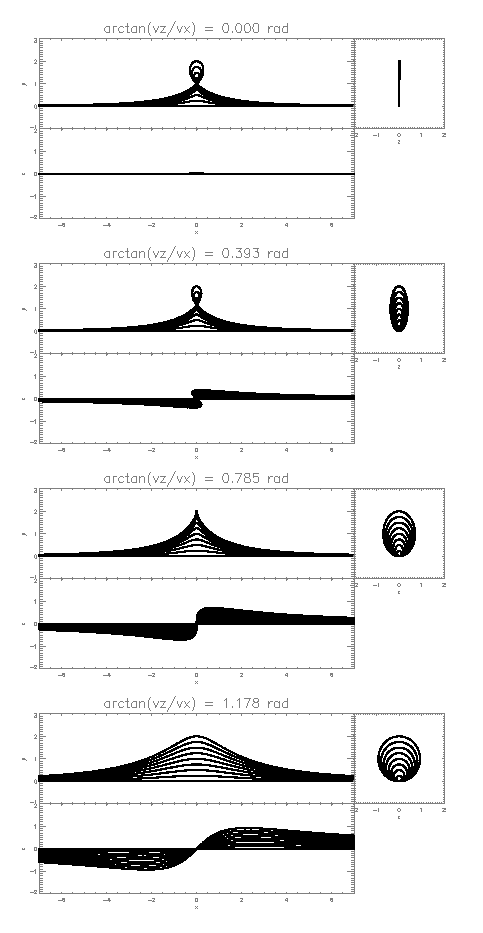
\includegraphics{grid.eps}
\end{center}
\caption{The perturbation of the stream in rotated, boosted, scaled
  coordinates, for four different angles $\theta=\arctan(v_z/v_x)$ and
  scaled times of $0$, $0.25$, \ldots, $2.0$.  See text for definition
  of scaled coordinates, scaled time, and angle.\label{fig:grid}}
\end{figure}

\clearpage
\begin{figure}
\begin{center}
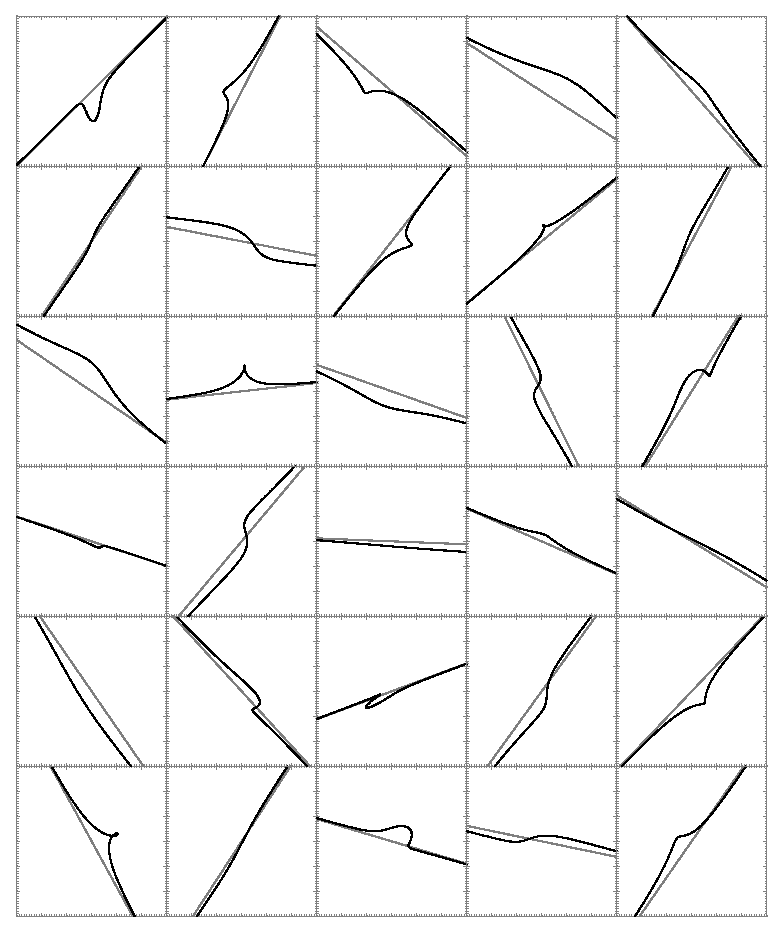
\includegraphics{views.eps}
\end{center}
\caption{Views of randomly generated perturbed streams, generated from
  a uniform angle distribution between $0$ and $2\pi$~rad and a
  uniform scaled time distribution between $0.25$ and $1.25$ projected
  onto randomly oriented planes.  Black shows the perturbed orbit and
  grey shows the unperturbed orbit.\label{fig:views}}
\end{figure}

\end{document}
